\documentclass[11pt,a4paper]{article}

\usepackage[utf8]{inputenc}
\usepackage[T1]{fontenc}
\usepackage{authblk}
\usepackage{graphicx}
\usepackage{float}
\usepackage{textgreek}
\usepackage{booktabs}
\usepackage{multirow}
\usepackage{caption}
\usepackage{xcolor}
\usepackage[colorlinks=true,citecolor=blue, linkcolor = blue, urlcolor=blue]{hyperref}
\usepackage{cite}

\usepackage[margin = 2.54cm]{geometry}

\setlength{\abovecaptionskip}{16pt}

\linespread{1} % Set linespace

\bibliographystyle{plos2025}


\title{\textbf{Supplementary material for Dos Santos \textit{et al}. (2025)}}

\author[$\dagger$ ]{Scott J. Dos Santos}
\author[$\dagger$ ]{Andreea C. Murariu}
\author[ ]{Justin D. Silverman}
\author[*]{Gregory B. Gloor}

\affil[$\dagger$]{Equal contribution}
\affil[*]{Corresponding author}

\date{November 2025}

%-----------------------
% Begin document
%-----------------------
\begin{document}

\maketitle

\section*{Contents}

\paragraph*{Fig. \ref{fig:supFigFDR_all}}
False-discovery and true-positive rates for all datasets tested.

\paragraph*{Fig. \ref{fig:supFigTPR_all}}
False-discovery and true-positive rates for all datasets tested.

\paragraph*{Fig. \ref{fig:supFigPPV_all}}
Positive predictive values for all datasets tested.

\paragraph*{Table \ref{tab:supTabDensity}}
Average minimum log differences required for a significant result with ALDEx2 and ALDEx3 for all datasets and \textgamma~values.

\paragraph*{Fig. \ref{fig:supFigDispAbund}}
Features from single-cell and metatranscriptome datasets have a larger dispersion compared to bulk RNA-seq data.

\paragraph*{Fig. \ref{fig:supFigDensity}}
ALDEx3 returns a tighter distribution of minimum log-difference values required for significance across all datasets.

\paragraph*{Table \ref{tab:sigGenesReal}}
Differentially expressed genes reported by all tested tools for the original, non-permuted BRCA dataset.

\paragraph*{Fig. \ref{fig:supFigEffect}}
Boundaries between features reported as differentially expressed at different \textgamma~values are curved.

\paragraph*{Fig. \ref{fig:supFigPTEN}}
Significant differences in \textit{PTEN} expression are driven by a few outlier samples.

\paragraph*{File \color{blue}{ S1}}
Genes dropped as scale uncertainty increases are largely unrelated to cancer development (available for download from article page and on GitHub: \url{https://github.com/amurariu/usri/blob/main/data/SupplementaryFile1_droppedALDEx.xlsx}).

\newpage

\renewcommand{\figurename}{\textbf{Supplementary Figure}}
\renewcommand{\thefigure}{\textbf{S\arabic{figure}}}


\renewcommand{\tablename}{\textbf{Supplementary Table}}
\renewcommand{\thetable}{\textbf{S\arabic{table}}}


\begin{figure}[H]
    \centering
    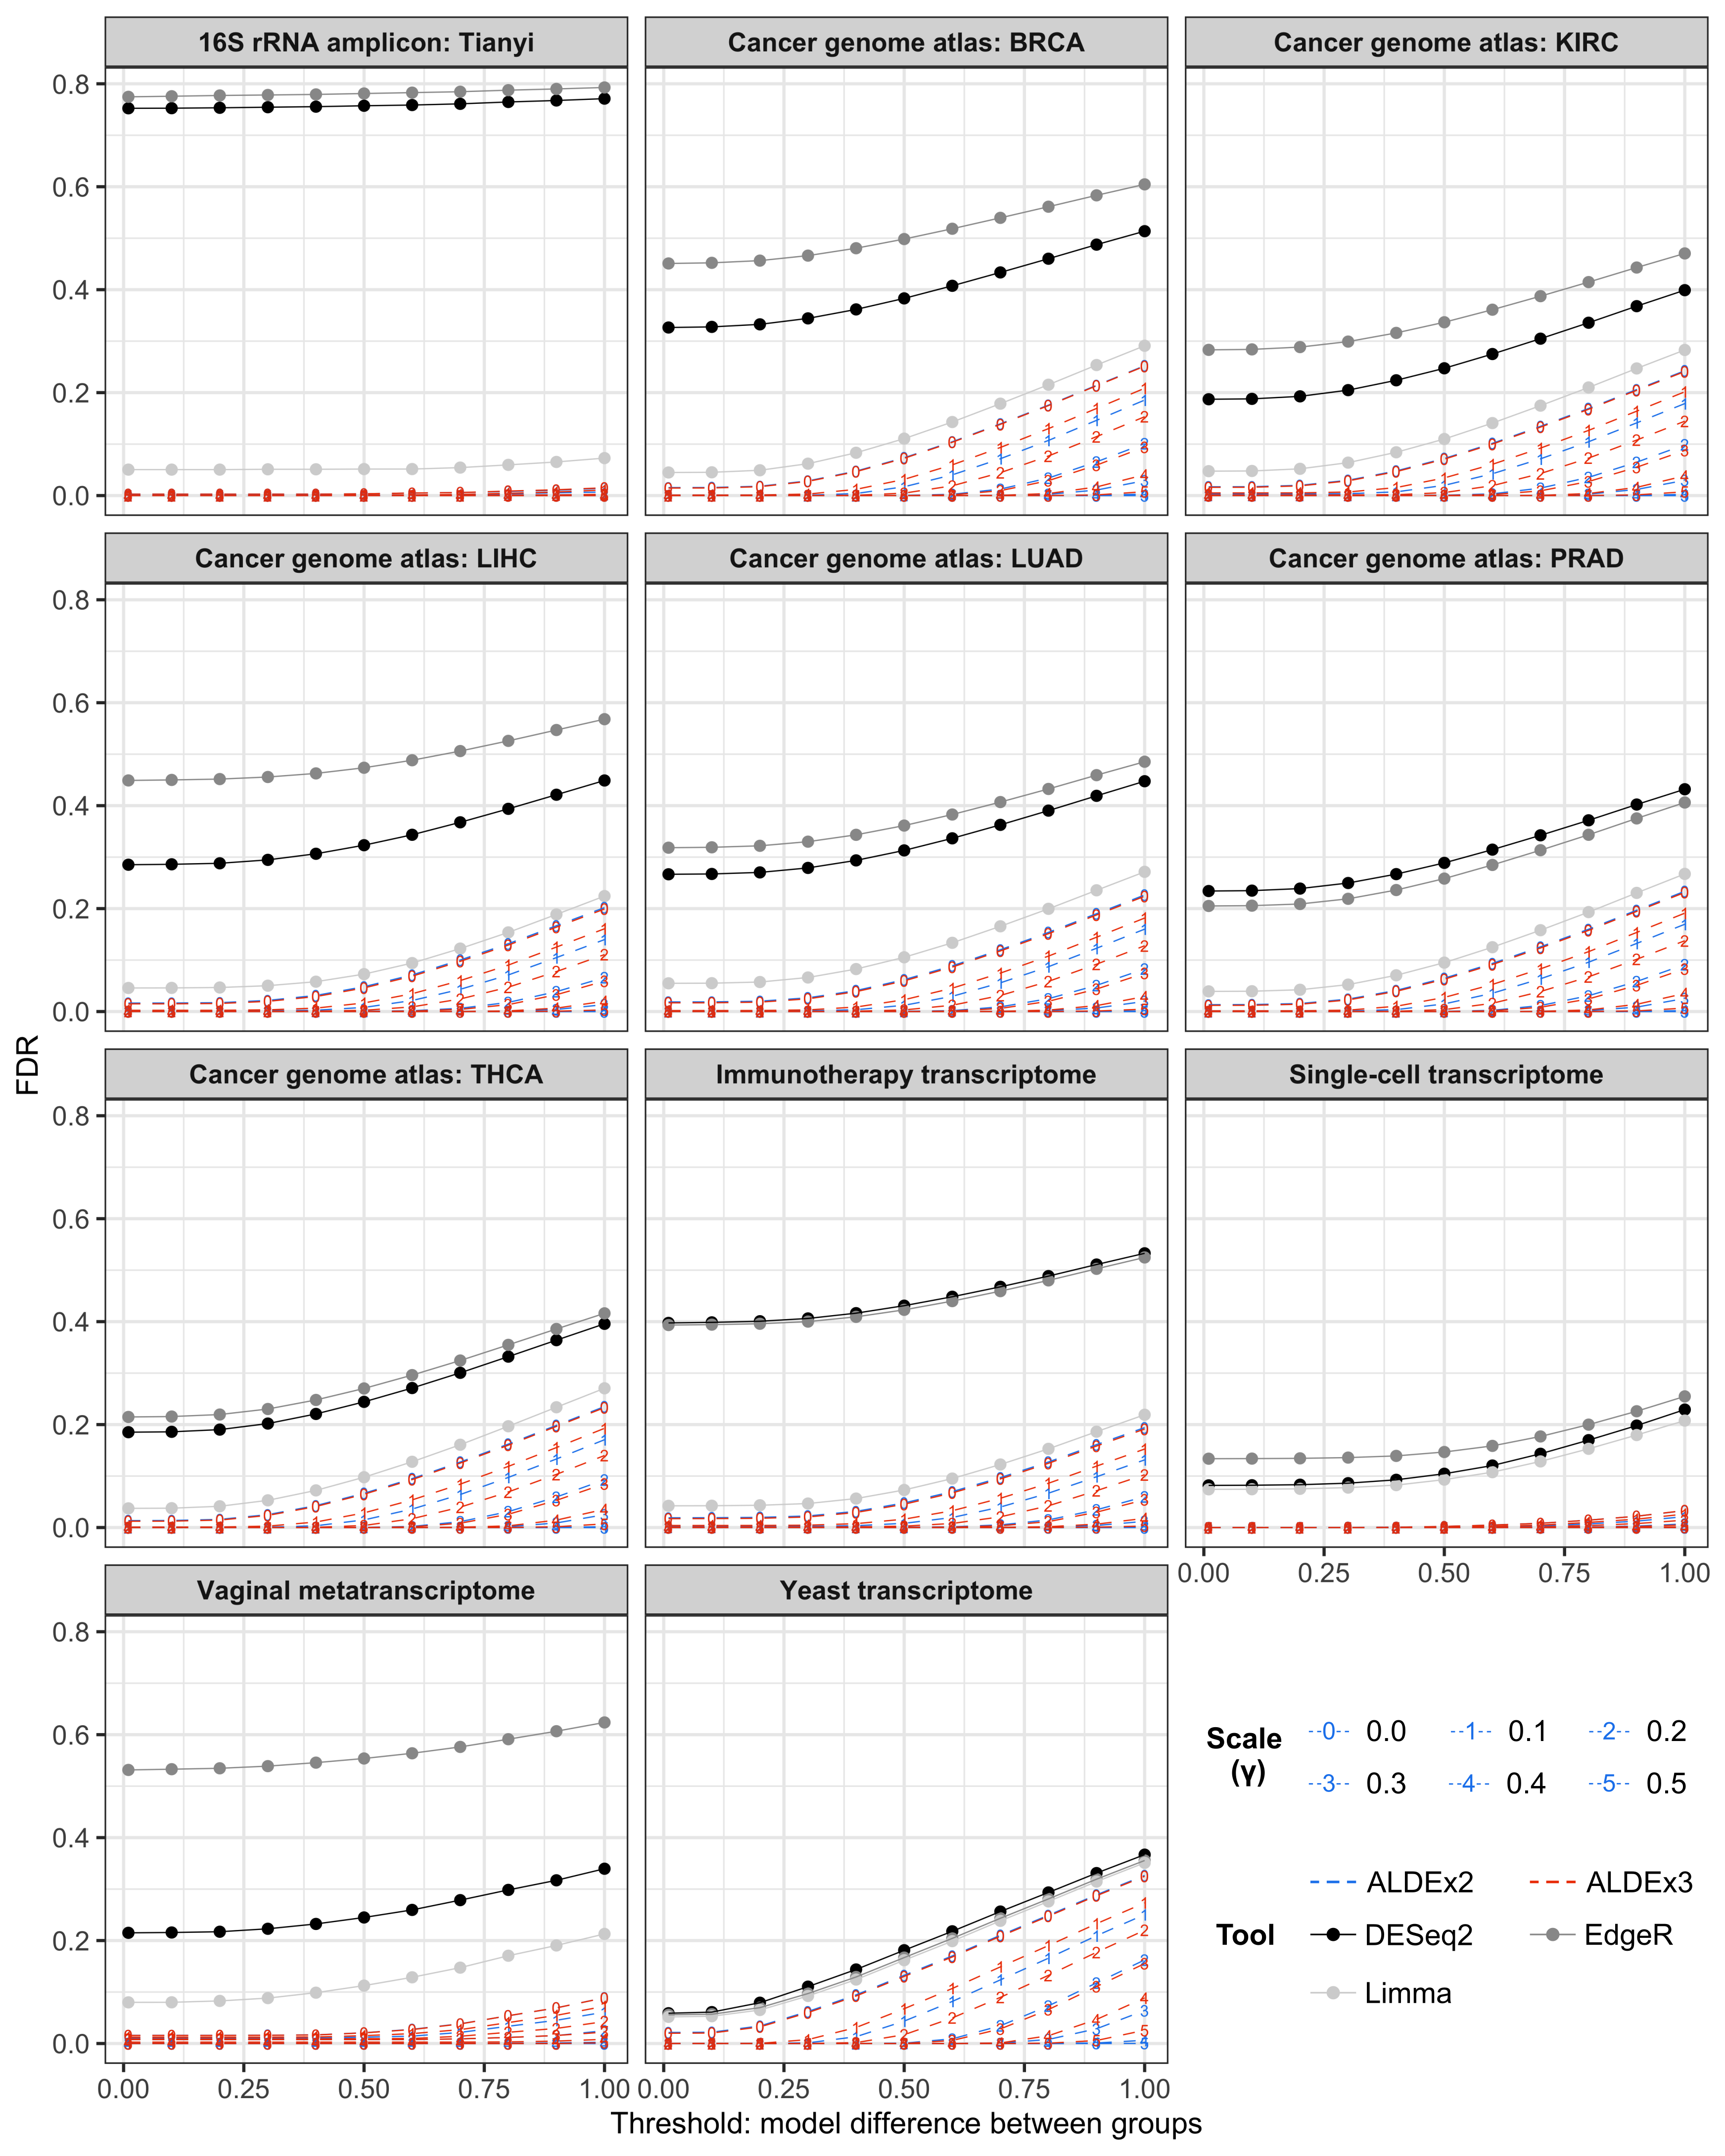
\includegraphics[width = \linewidth]{supFig_FDR_all.png}
\caption{\textbf{False-discovery rates for all datasets tested.} False-discovery rates (FDR) for all tool and dataset combinations were calculated separately for each 0.1 increment in the model difference between groups (i.e. the simulated or `true' log\textsubscript{2} fold-change between groups, as determined by binomial thinning). Each data point represents the FDR when considering dataset features with a simulated log-difference at or above the given x-axis threshold. Features were considered differentially abundant at a BH-adjusted \textit{P}-value of $<$0.05.}
    \label{fig:supFigFDR_all}
\end{figure}
\newpage

\begin{figure}[H]
    \centering
    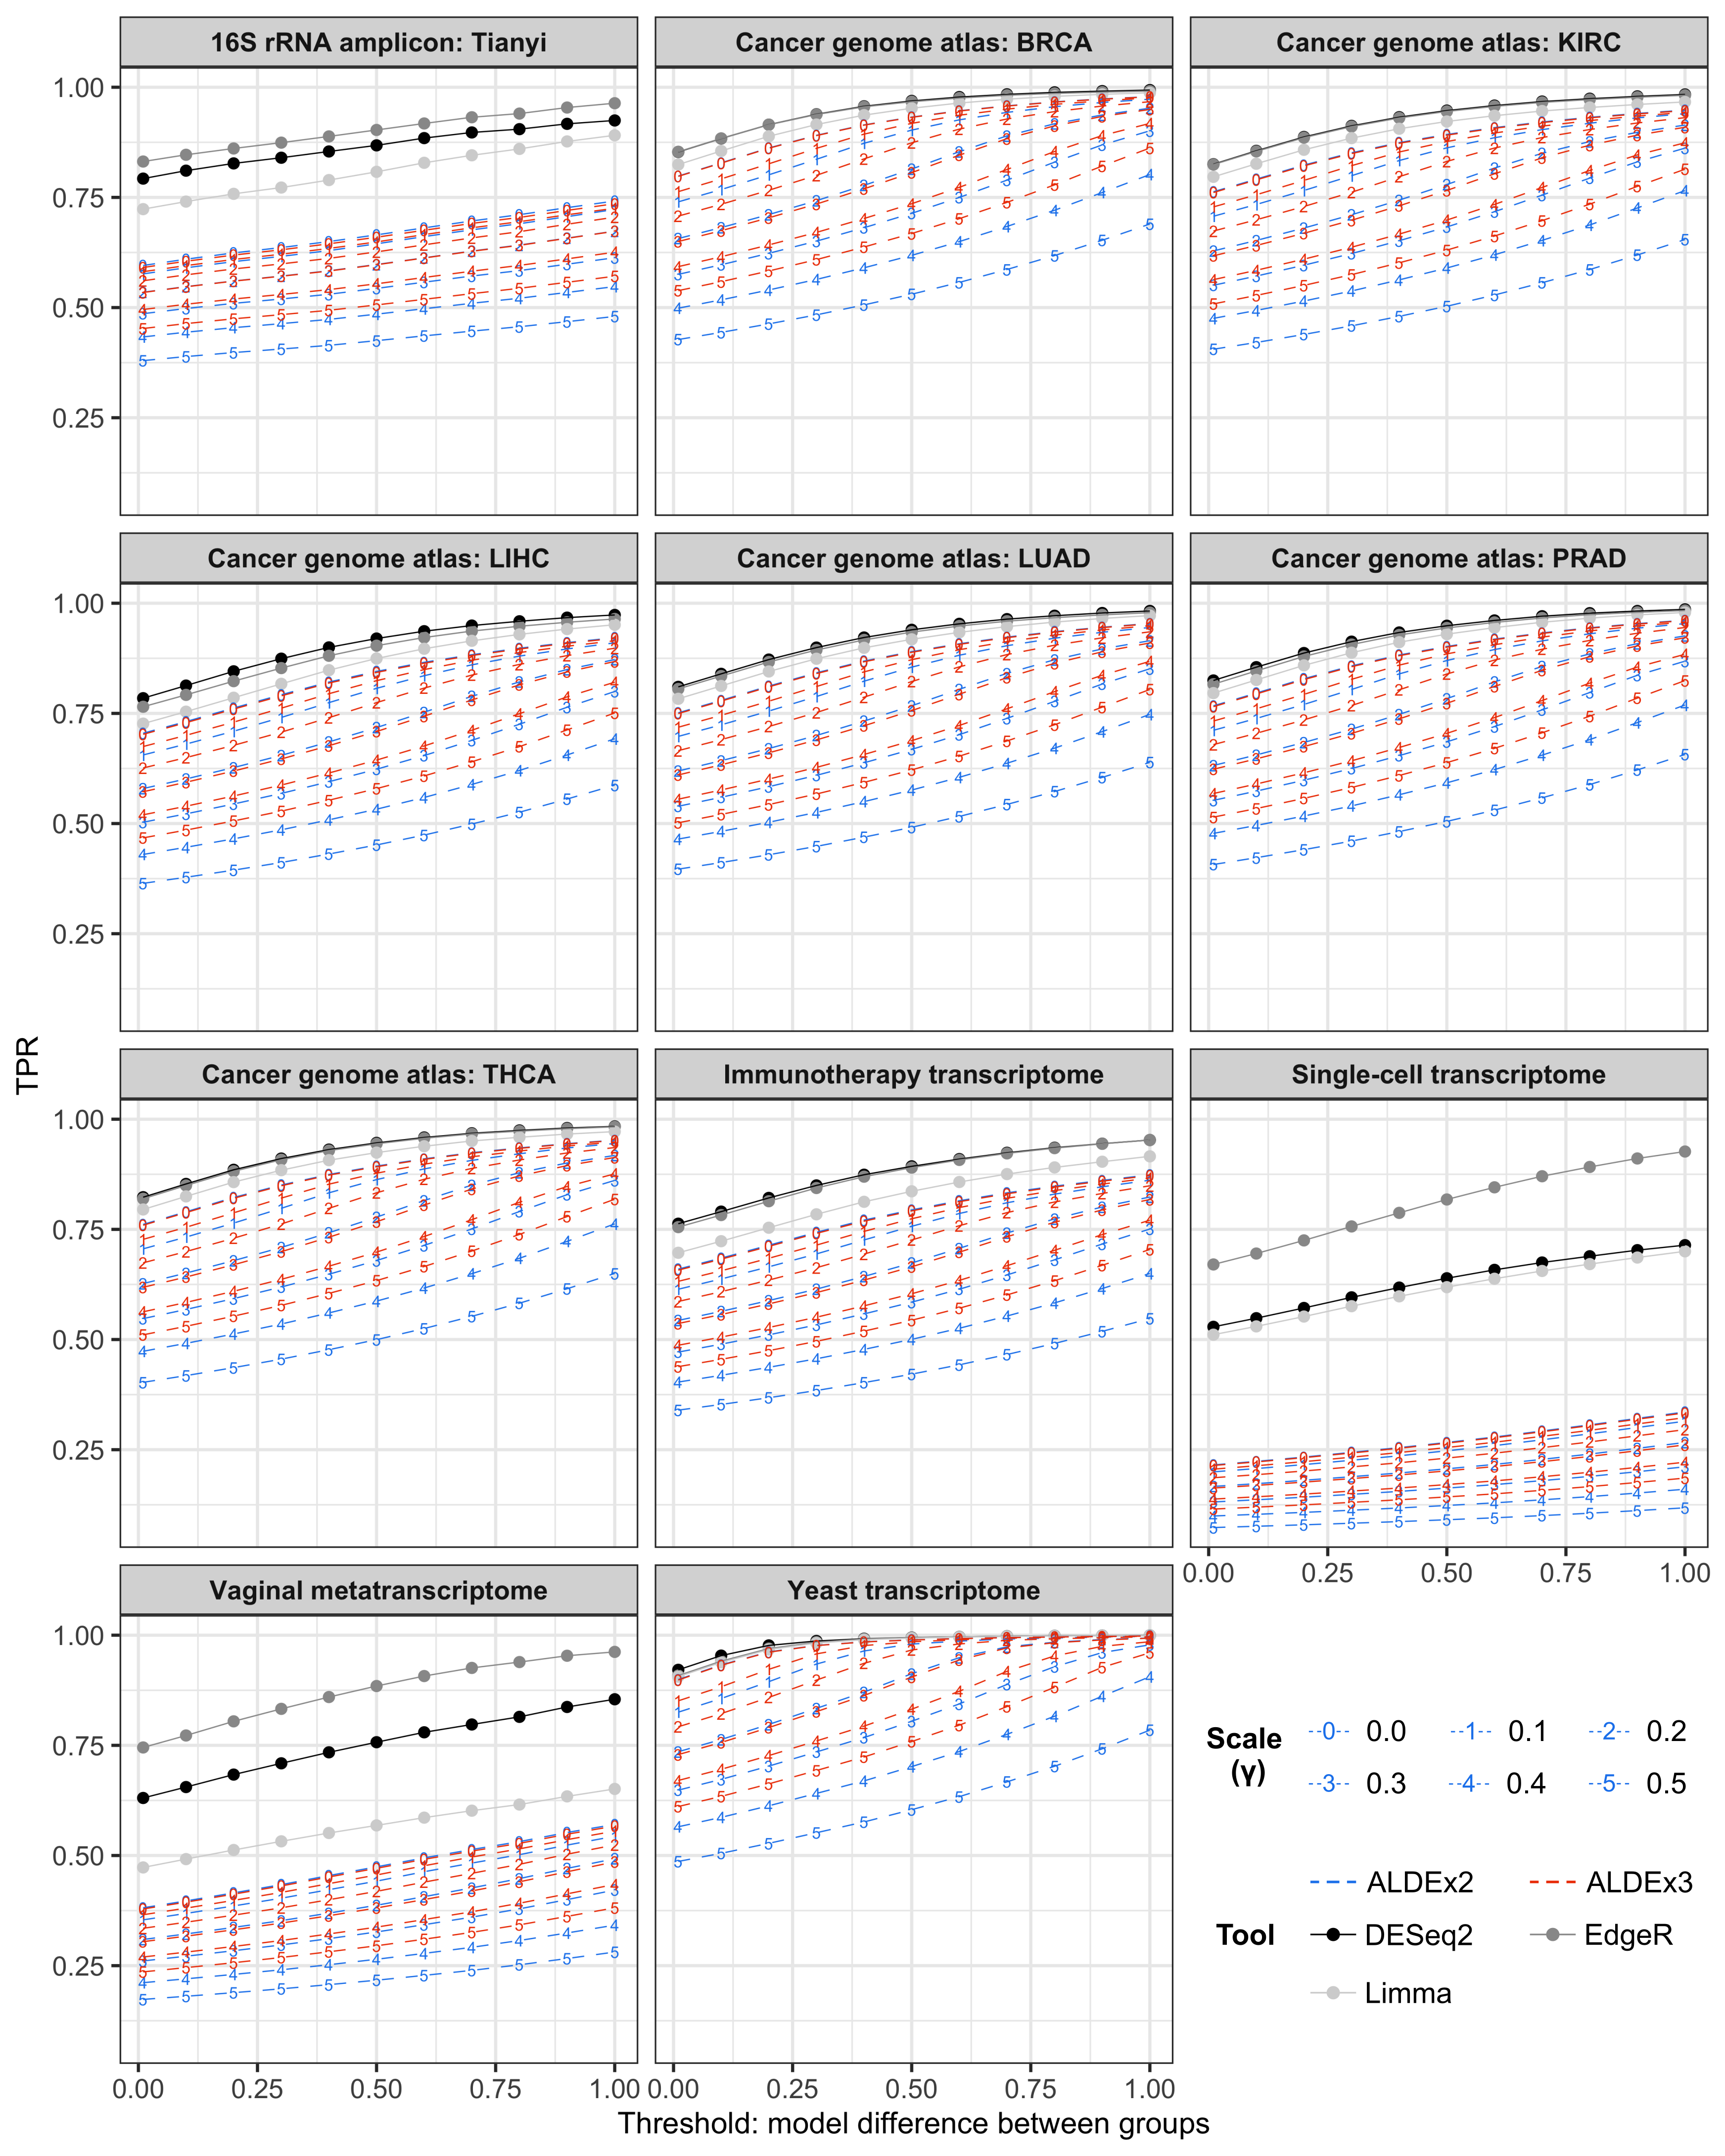
\includegraphics[width = \linewidth]{supFig_TPR_all.png}
\caption{\textbf{False-discovery and true-positive rates for all datasets tested.} True positive rates (TPR) for all tool and dataset combinations were calculated separately for each 0.1 increment in the model difference between groups (i.e. the simulated or `true' log\textsubscript{2} fold-change between groups, as determined by binomial thinning). Each data point represents the TPR when considering dataset features with a simulated log-difference at or above the given x-axis threshold. Features were considered differentially abundant at a BH-adjusted \textit{P}-value of $<$0.05.}
    \label{fig:supFigTPR_all}
\end{figure}
\newpage

\begin{figure}[H]
    \centering
    
\includegraphics[width = \linewidth]{supFig_PPV_all.png}
    \caption{\textbf{Positive predictive values for all datasets tested.} The positive predictive value (PPV) for all tool and dataset combinations was calculated separately for each 0.1 increment in the model difference between groups (i.e. the simulated or `true' log\textsubscript{2} fold-change between groups, as determined by binomial thinning). Each data point represents the PPV when considering dataset features with a simulated log-difference at or above the given x-axis threshold. Features were considered differentially abundant at a BH-adjusted \textit{P}-value of $<$0.05.}
    \label{fig:supFigPPV_all}
\end{figure}
\newpage

\begin{table}[H]
    \caption{\textbf{Average minimum log differences required for a significant result with ALDEx2 and ALDEx3 for all datasets and \textgamma~values:} For all datasets, the mean minimum log difference required for ALDEx2 and ALDEx3 to recognise a feature as differentially expressed (i.e. BH-adjusted \textit{P}-value $<$0.05) was calculated for \textgamma~values ranging from 0 to 0.5. Data represent a mean of all 100 iterations of permuted/thinned count data (TGCA, The Cancer Genome Atlas).}
    \centering
    \begin{tabular}{ccrr}
         \toprule
         & & \multicolumn{2}{c}{Mean minimum difference ($\pm$~s.d.)}\\
         \cmidrule(lr){3-4}
         Dataset & Scale (\textgamma) & ALDEx2 & ALDEx3\\
         \midrule
         \multirow{6}{*}{Immunotherapy} & 0 & \textbf{0.34} (0.045) & \textbf{0.36} (0.041)\\
          & 0.1 & \textbf{0.54} (0.044) & \textbf{0.48} (0.040)\\
          & 0.2 & \textbf{0.78} (0.059) & \textbf{0.64} (0.040)\\
          & 0.3 & \textbf{1.02} (0.079) & \textbf{0.80} (0.051)\\
          & 0.4 & \textbf{1.27} (0.108) & \textbf{0.98} (0.061)\\
          & 0.5 & \textbf{1.52} (0.132) & \textbf{1.14} (0.070)\\
          \midrule
         \multirow{6}{*}{Metatranscriptome} & 0 & \textbf{0.96} (0.261) & \textbf{0.96} (0.260)\\
          & 0.1 & \textbf{1.10} (0.246) & \textbf{1.04} (0.257)\\
          & 0.2 & \textbf{1.35} (0.280) & \textbf{1.21} (0.245)\\
          & 0.3 & \textbf{1.59} (0.275) & \textbf{1.37} (0.271)\\
          & 0.4 & \textbf{1.90} (0.327) & \textbf{1.57} (0.291)\\
          & 0.5 & \textbf{2.16} (0.376) & \textbf{1.76} (0.291)\\
          \midrule
         \multirow{6}{*}{Single-cell} & 0 & \textbf{0.85} (0.213) & \textbf{0.93} (0.250)\\
          & 0.1 & \textbf{1.00} (0.202) & \textbf{1.01} (0.233)\\
          & 0.2 & \textbf{1.21} (0.191) & \textbf{1.18} (0.230)\\
          & 0.3 & \textbf{1.45} (0.199) & \textbf{1.34} (0.222)\\
          & 0.4 & \textbf{1.73} (0.208) & \textbf{1.53} (0.225)\\
          & 0.5 & \textbf{2.01} (0.253) & \textbf{1.72} (0.235)\\
          \midrule
         \multirow{6}{*}{TCGA} & 0 & \textbf{0.24} (0.056) & \textbf{0.25} (0.055)\\
          & 0.1 & \textbf{0.45} (0.051) & \textbf{0.39} (0.049)\\
          & 0.2 & \textbf{0.69} (0.068) & \textbf{0.55} (0.053)\\
          & 0.3 & \textbf{0.93} (0.089) & \textbf{0.72} (0.060)\\
          & 0.4 & \textbf{1.17} (0.113) & \textbf{0.88} (0.068)\\
          & 0.5 & \textbf{1.41} (0.140) & \textbf{1.05} (0.077)\\
          \midrule
         \multirow{6}{*}{Tianyi 16S rRNA} & 0 & \textbf{1.81} (0.551) & \textbf{1.91} (0.552)\\
          & 0.1 & \textbf{1.89} (0.523) & \textbf{1.96} (0.525)\\
          & 0.2 & \textbf{2.07} (0.497) & \textbf{2.07} (0.549)\\
          & 0.3 & \textbf{2.30} (0.518) & \textbf{2.19} (0.533)\\
          & 0.4 & \textbf{2.50} (0.507) & \textbf{2.35} (0.519)\\
          & 0.5 & \textbf{2.79} (0.684) & \textbf{2.61} (0.632)\\
          \midrule
         \multirow{6}{*}{Yeast} & 0 & \textbf{0.18} (0.046) & \textbf{0.18} (0.046)\\
          & 0.1 & \textbf{0.39} (0.045) & \textbf{0.32} (0.040)\\
          & 0.2 & \textbf{0.63} (0.065) & \textbf{0.47} (0.044)\\
          & 0.3 & \textbf{0.87} (0.087) & \textbf{0.65} (0.056)\\
          & 0.4 & \textbf{1.11} (0.113) & \textbf{0.81} (0.062)\\
          & 0.5 & \textbf{1.35} (0.147) & \textbf{0.98} (0.069)\\
         \bottomrule
    \end{tabular}
    \label{tab:supTabDensity}
\end{table}
\newpage

\begin{figure}[H]
    \centering
    
\includegraphics[width=\linewidth]{supFig_dispersionAbundance.png}
    \caption{\textbf{Features from single-cell and metatranscriptome datasets have a larger dispersion compared to bulk RNA-seq data.} The within-group log dispersion of each feature was plotted against its log abundance. Data were sourced from a single, randomly selected iteration of the ALDEx2 permutation analyses from each dataset.}
    \label{fig:supFigDispAbund}
\end{figure}
\newpage

\begin{figure}[H]
    \centering
    
\includegraphics[width=\linewidth]{supFig_densityPlotsALDEx_otherDatasets.png} 
    \caption{\textbf{ALDEx3 returns a tighter distribution of minimum log-difference values required for significance across all datasets.} For each of the 100 iterations of the given dataset, the minimum absolute difference between groups needed for a gene to be reported as differentially expressed by ALDEx2 and ALDEx3 was recorded, based on a BH-adjusted \textit{P}-value of $<$0.05, for \textgamma~values ranging from 0 to 0.5. Data for the Cancer Genome Atlas (TCGA), vaginal metatranscriptome, single-cell, 16S rRNA amplicon, and yeast transcriptome datasets are expressed as density plots and coloured by tool and \textgamma~value. Values for TCGA datasets represent an aggregate across the individual tumour transcriptome datasets. Dashed lines indicate the mean value.}
    \label{fig:supFigDensity}
\end{figure}
\newpage


\begin{table}[H]
    \caption{\textbf{Differentially expressed genes reported by all tested tools for the original, non-permuted BRCA dataset:} The total number of genes identified as differentially expressed by ALDEx2 (A2), ALDEx3 (A3), DESeq2 (DS), edgeR (ER) and limma-voom (LM) are shown for increasing values of \textgamma. At each \textgamma~value from 0.1 to 0.5, the number and proportion of genes belonging to the `canonical drivers' and `breast cancer' categories of the Network of Cancer Genes \cite{repana_network_2019} that are no longer significantly different between groups (i.e. dropped genes) are also shown for ALDEx2 and ALDEx3. Data represent the results of a single analysis performed with the original, non-permuted count table and group membership vector. Dashes indicate non-applicable fields.}
    \centering
    \begin{tabular}{crrrrrrr}
        \toprule
        & \multicolumn{5}{c}{No. differentially expressed genes} & \multicolumn{2}{c}{No. dropped NCG genes}\\
        \cmidrule(lr){2-6} \cmidrule(lr){7-8}
        \textgamma{} & A2 & A3 & DS & ER & LM & A2 & A3 \\
        \midrule
        0 & 15,837 & 15,825 & 16,736 & 16,407 & 16,295 & - & - \\
        0.1 & 12,959 & 13,696 & - & - & - & 24 (0.83) & 18 (0.85) \\
        0.2 & 8,976 & 10,754 & - & - & - & 18 (0.45) & 12 (0.41) \\
        0.3 & 5,857 & 8,097 & - & - & - & 17 (0.55) & 17 (0.64) \\
        0.4 & 3,956 & 5,966 & - & - & - & 16 (0.84) & 12 (0.56) \\
        0.5 & 2,777 & 4,437 & - & - & - & 7 (0.59) & 14 (0.92) \\
        \bottomrule
    \end{tabular}
    \label{tab:sigGenesReal}
\end{table}
\newpage

\begin{figure}[H]
    \centering
    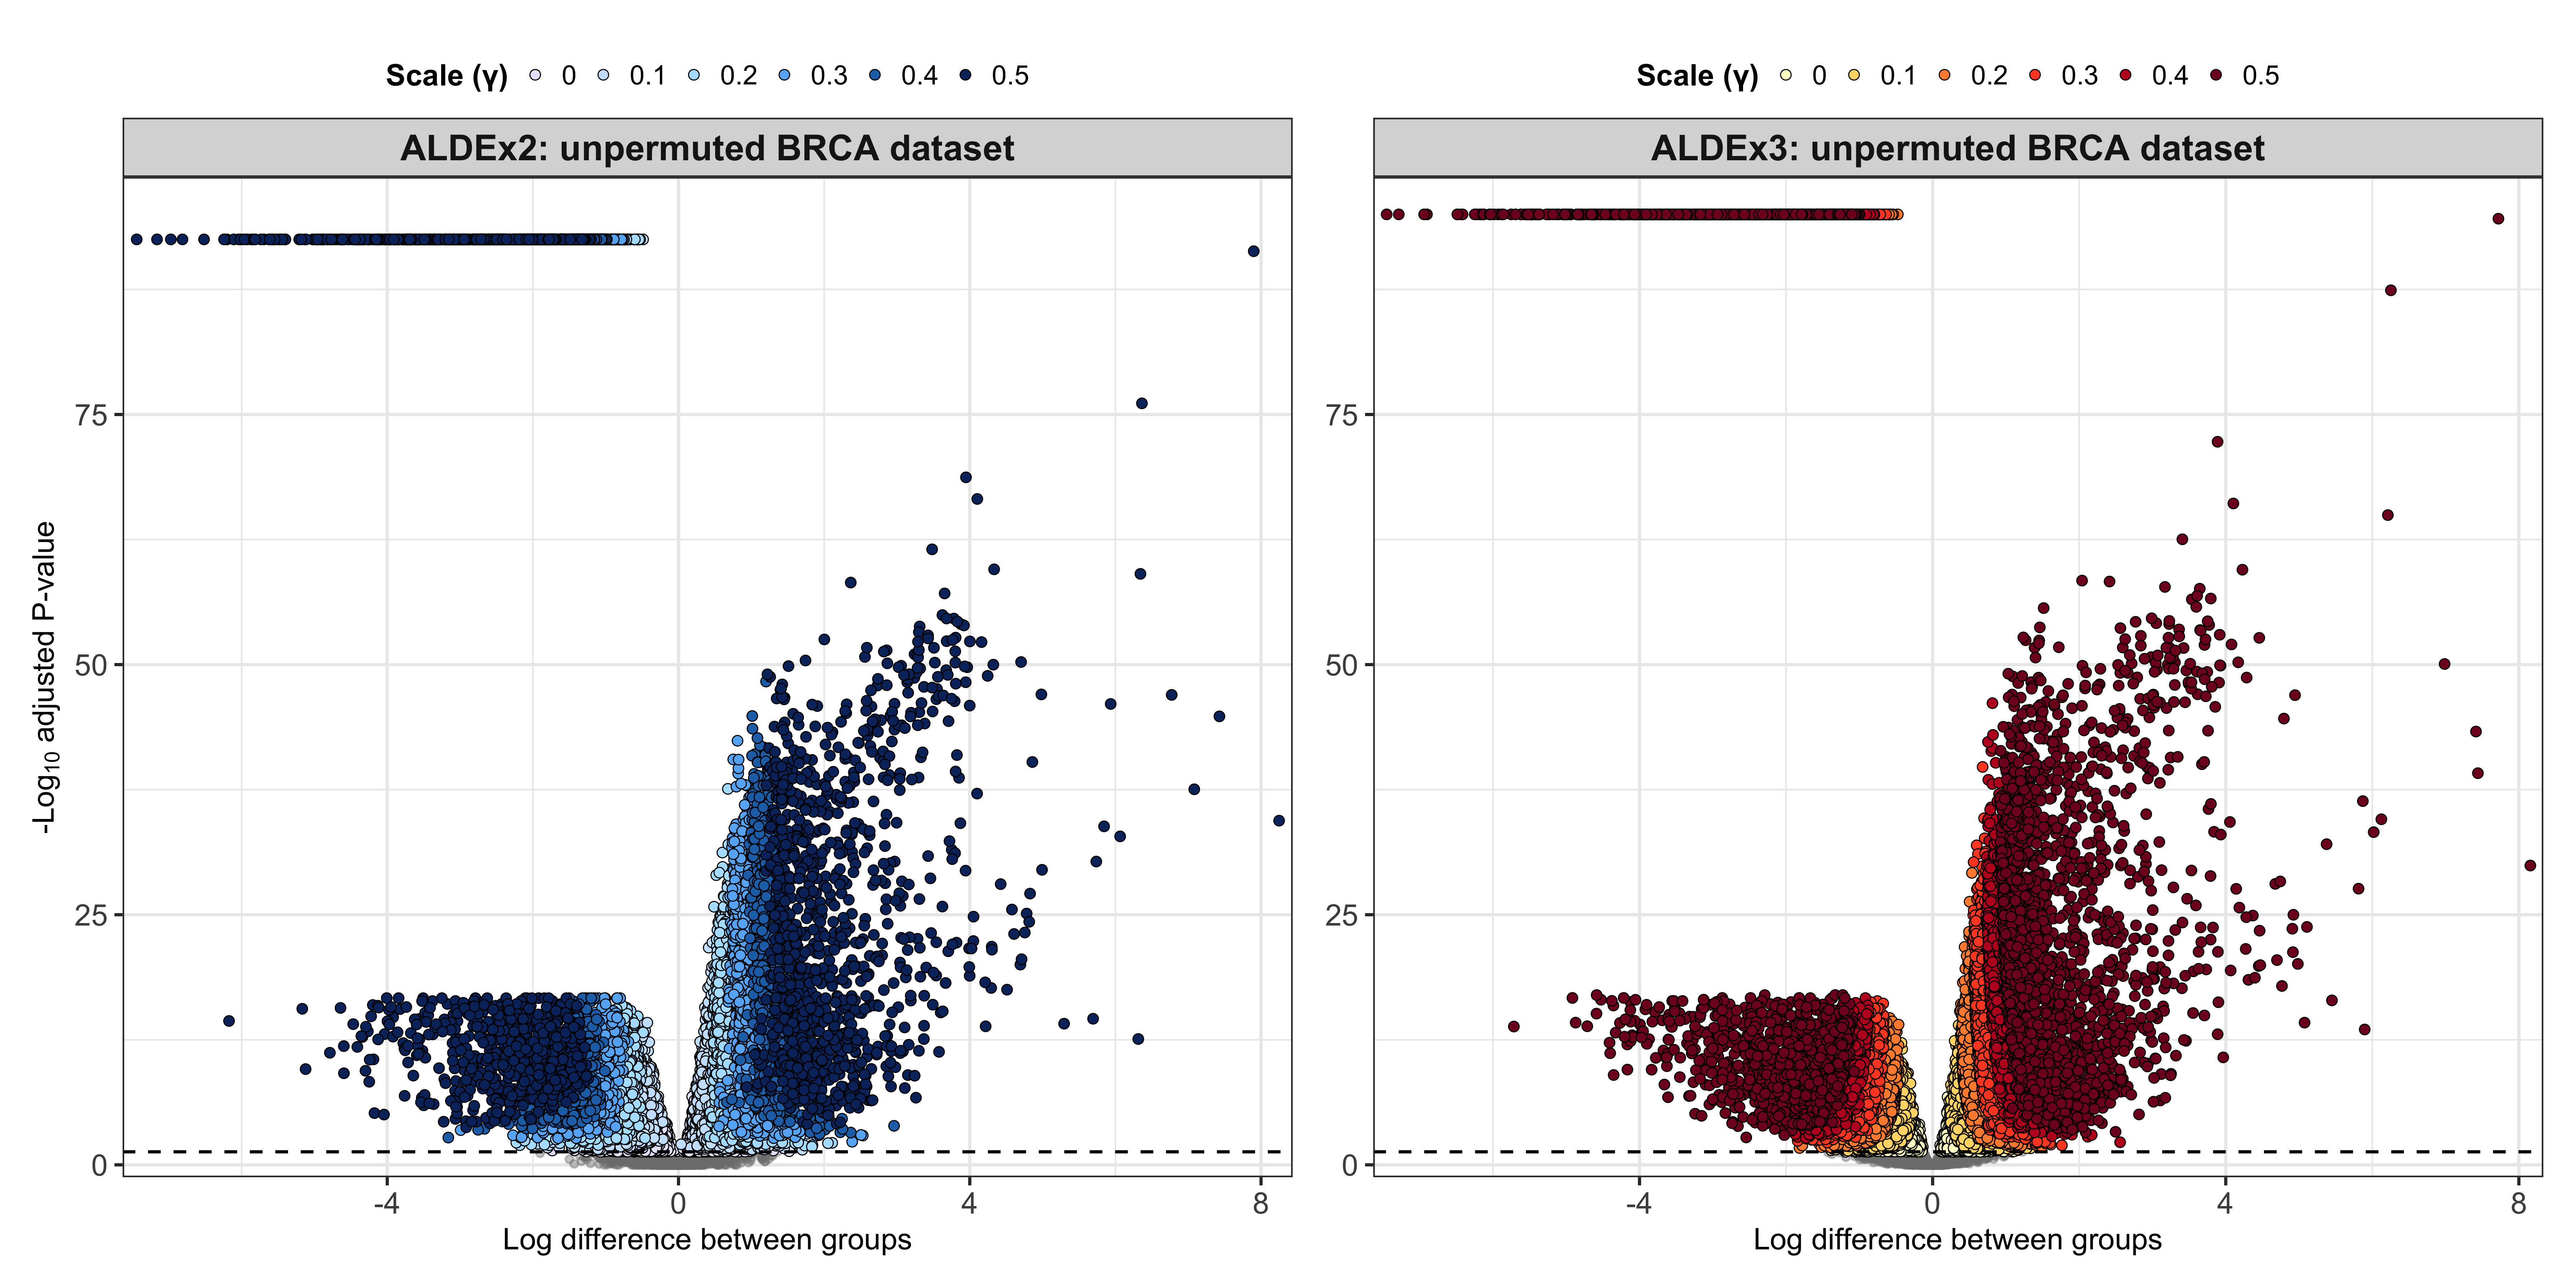
\includegraphics[width=\linewidth]{supFig_effectBorders.png}
    \caption{\textbf{Boundaries between features reported as differentially expressed at different \textgamma~values are curved:} Volcano plots of log difference between groups vs. -log\textsubscript{10} BH-adjusted \textit{P}-values were generated for ALDEx2 (\textbf{left}) and ALDEx3 (\textbf{right}) analyses of the original, non-permuted BRCA dataset from the Cancer Genome Atlas. Curved boundaries between points identified as differentially expressed at different \textgamma~values can be clearly seen. Each data point represents a feature from the scale-na\"ive analysis (\textgamma~= 0.001). Grey points indicate non-significant features; coloured points indicate features which are significantly different after a certain amount of scale uncertainty has been added to the model. Grey dashed lines indicate BH-adjusted \textit{P}-value $<$0.05.}
    \label{fig:supFigEffect}
\end{figure}
\newpage

\begin{figure}[H]
    \centering
    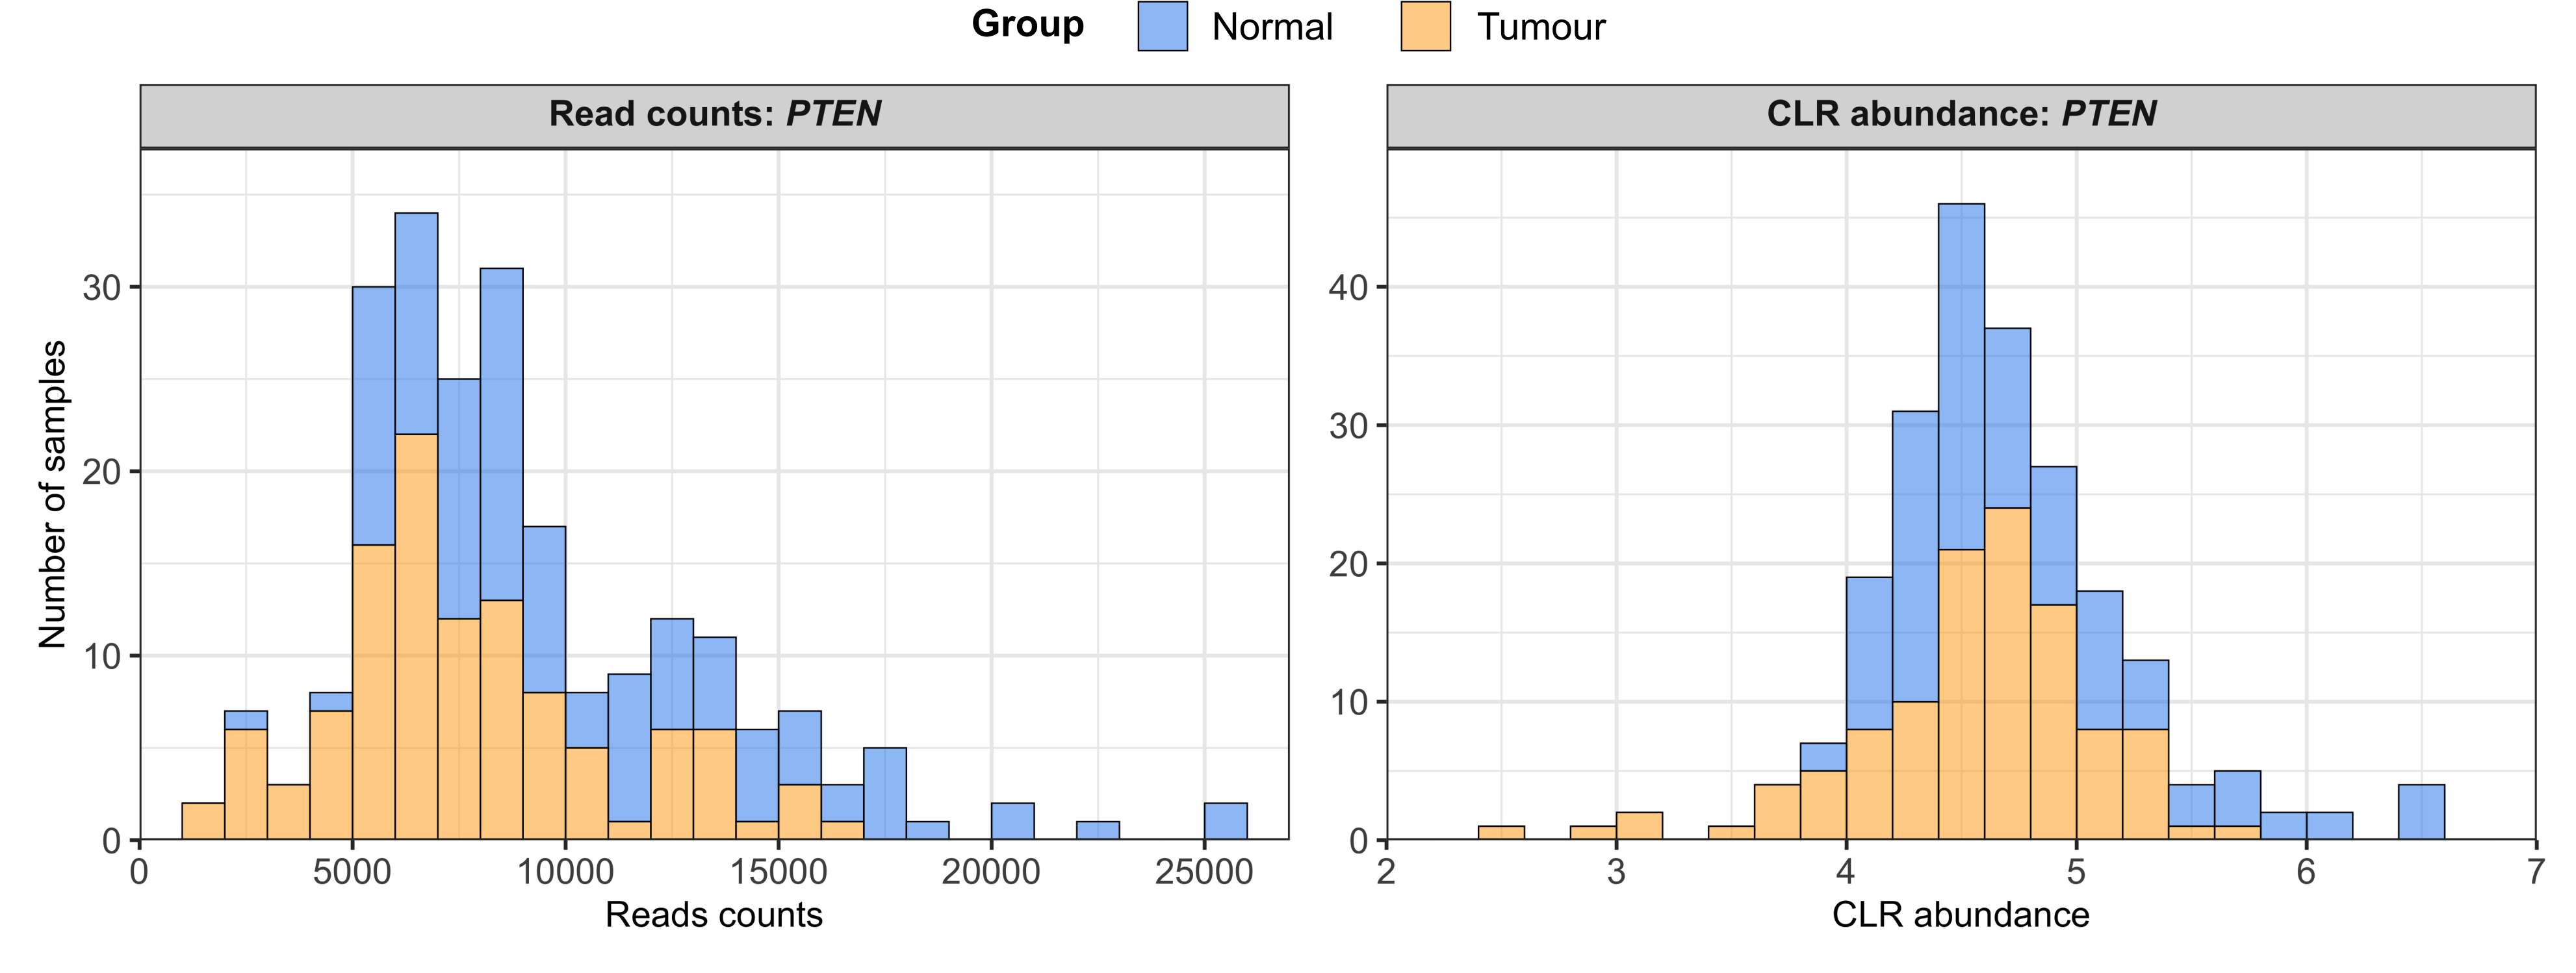
\includegraphics[width=\linewidth]{supFig_PTEN_distribution.png}
    \caption{\textbf{Significant differences in \textit{PTEN} expression are driven by a few outlier samples:} Expression of the tumour suppressor gene, \textit{PTEN}, in the Cancer Genome Atlas BRCA dataset is shown in histograms of read counts (\textbf{left}) and centred log-ratio (CLR) abundance values (\textbf{right}) calculated by ALDEx2. Bars are coloured by sample group. Bin width is 1,000 (reads) or 0.2 (CLR). The limited number of outlier samples in each group can clearly be seen at either end of the histograms, with most samples overlapping in the centre.}
    \label{fig:supFigPTEN}
\end{figure}
\newpage

\bibliography{diffAbund_refs.bib}

\end{document}